\documentclass[dvipdfmx, border=0pt]{standalone}
\usepackage{tikz}
\usetikzlibrary{calc}

\begin{document}
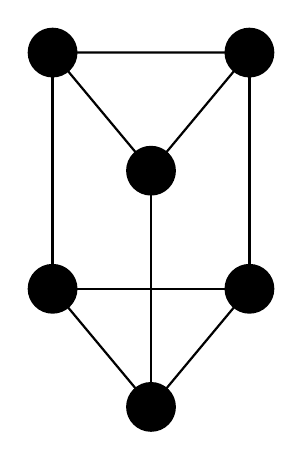
\begin{tikzpicture}[
  vertex/.style={circle, fill=black, inner sep=0pt, minimum size=18pt},
  edge/.style={thick},
  hidden edge/.style={thick, dashed, gray}
]

\coordinate (B1) at (0, 1);
\coordinate (B2) at (2.5, 1);
\coordinate (B3) at (1.25, -0.5);
\coordinate (T1) at ($(B1)+(0, 3)$);
\coordinate (T2) at ($(B2)+(0, 3)$);
\coordinate (T3) at ($(B3)+(0, 3)$);
\draw[edge] (B1) -- (B2);
\draw[edge] (B1) -- (B3) -- (B2);
\draw[edge] (B1) -- (T1);
\draw[edge] (B2) -- (T2);
\draw[edge] (B3) -- (T3);
\draw[edge] (T1) -- (T2) -- (T3) -- cycle;
\foreach \v in {B1, B2, B3, T1, T2, T3} {
  \node[vertex] at (\v) {};
}
\end{tikzpicture}
\end{document}